\documentclass[aspectratio=1610,compress,t,gabaritb,french,english]{hecppt}

%% Packages
\usepackage{fontawesome}
\usepackage{metalogo}
\usepackage{hyperref} % Ce package doit TOUJOURS être en dernier!

%% Options des packages
\frenchbsetup{og=«,fg=»}
\hypersetup{colorlinks=true,%
	urlcolor=bleuFoncePrimaire,%
	linkcolor=bleuFoncePrimaire,%
	pdfauthor=Votre Nom,%
	pdftitle=Titre de la présentation}

%% Commandes internes
\newcommand{\HEClien}[2]{%
	\href{#1}{\textbf{#2} \faExternalLink}
}

%% Métadonnées du document

\title{Writing tools for {\LaTeX}}
\subtitle{Tools from the Library and beyond}
\HECauteur{Benoit Hamel}{Benoit Hamel}
\date[]{\today}
\subject{} % Sujet inséré dans les métadonnées du pdf
\keywords{} % Mots-clés insérés dans les métadonnées du pdf

\begin{document}

\pageTitre

\begin{frame}[c]	
	\begin{center}
		The content of this presentation is licensed under the following terms :
	\end{center}		
	
\includegraphics[width=\textwidth]{licence.png}
	\begin{center}	
		\HEClien{https://creativecommons.org/licenses/by-nc-sa/4.0/}{View the license}
	\end{center}
\end{frame}

\begin{frame}[c]{Contents}
	\tableofcontents
\end{frame}

\section{Tools made by the Library}

	\subsection{hecthese document class}
	
		\begin{frame}[c,fragile]{hecthese document class}
			\framesubtitle{What is it?}
			
			\begin{itemize}
				\item Framework for writing your dissertation at HEC Montréal;
				\item Includes :
				\begin{itemize}
					\item A class definition file;
					\item Two dissertation templates;
					\item All necessary accompanying files;
					\item A 25-pages documentation.
				\end{itemize}
				\item Complies with all 
					\HEClien{http://www.hec.ca/qualitecomm/anglais/ressources/guide-redaction-depot-memoire-anglais.pdf}%
					{presentation standards} required by the University.
			\end{itemize}
		\end{frame}
	
		\begin{frame}{hecthese document class}
			\framesubtitle{Where can we find it?}
			
			\begin{HECimagesstitre}{\centering https://ctan.org/pkg/hecthese}
				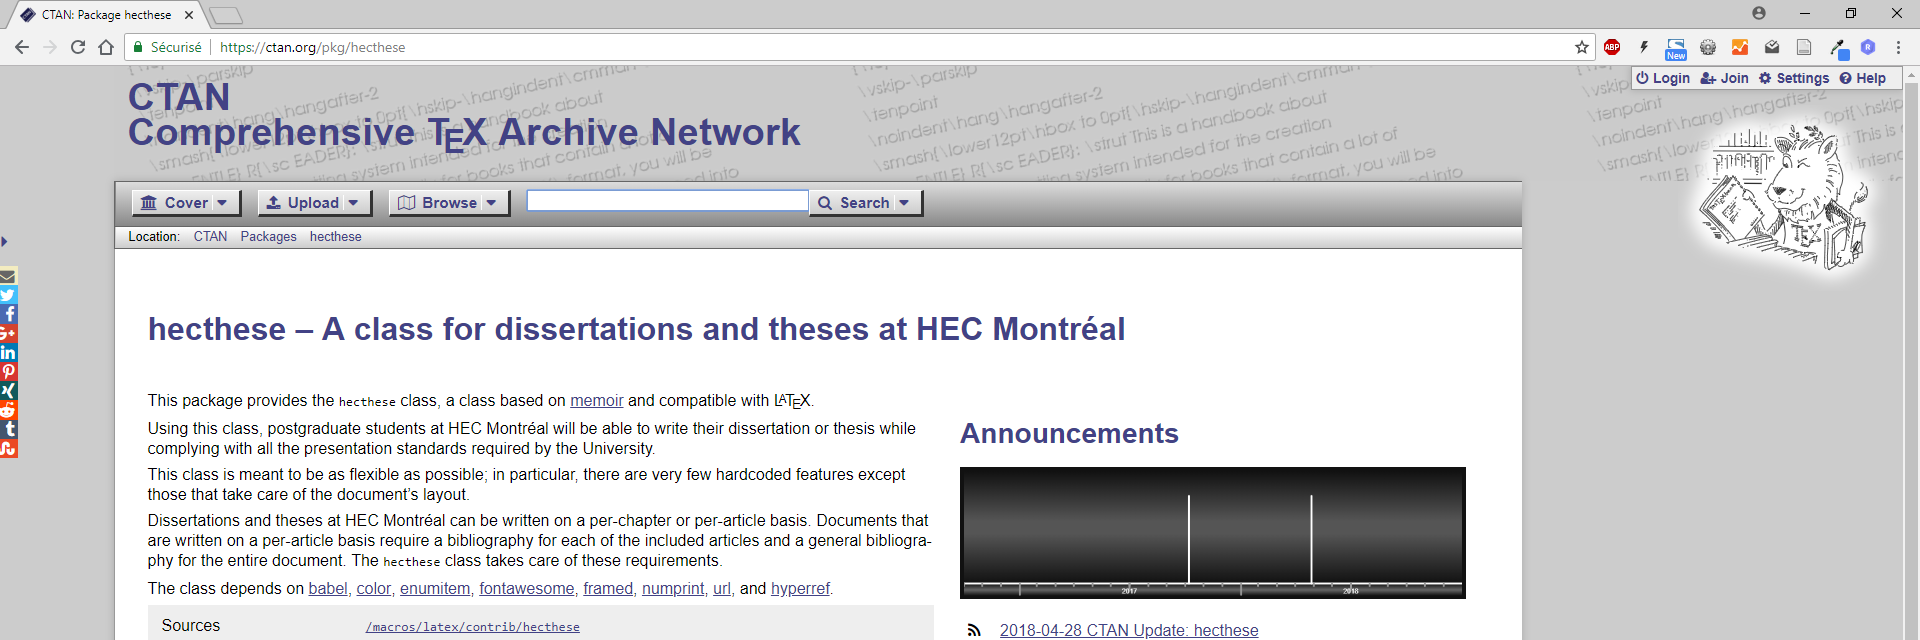
\includegraphics[width=\textwidth]{ctan-hecthese.png}
			\end{HECimagesstitre}
		\end{frame}
	
		\begin{frame}[c]{hecthese document class}
			\framesubtitle{How do we work with it?}
			\begin{itemize}
				\item Download the package from the \HEClien{https://ctan.org/pkg/hecthese}{CTAN website};
				\item Install the package files in a working directory
					(\HEClien{https://www.youtube.com/watch?v=nfTEgcJbufs}{video tutorial});
				\item Choose a template;
				\item Write your dissertation sections in each designated file;
				\item Compile your document from the template.
			\end{itemize}
		\end{frame}

	\subsection{hecppt document class}
	
		\begin{frame}{hecppt document class}
			\framesubtitle{What is it?}
			
			\begin{itemize}
				\item Document class for creating \HEClien{https://ctan.org/pkg/beamer}{beamer presentations}
					with the HEC Montréal trademark;
				\item Includes :
				\begin{itemize}
					\item A class definition file;
					\item A template file;
					\item All necessary accompaniyng files;
					\item A 21-pages documentation.
				\end{itemize}
				\item Complies with all \HEClien{http://marque.hec.ca/}{presentation standards}
					of the HEC Montréal trademark;
				\item Public beta phase: the package is fully functional but still in development stage.
			\end{itemize}
		\end{frame}
		
		\begin{frame}{hecppt document class}
			\framesubtitle{Where can we find it?}
			
			\begin{HECimagesstitre}{\centering https://github.com/metalogueur/hecppt}
				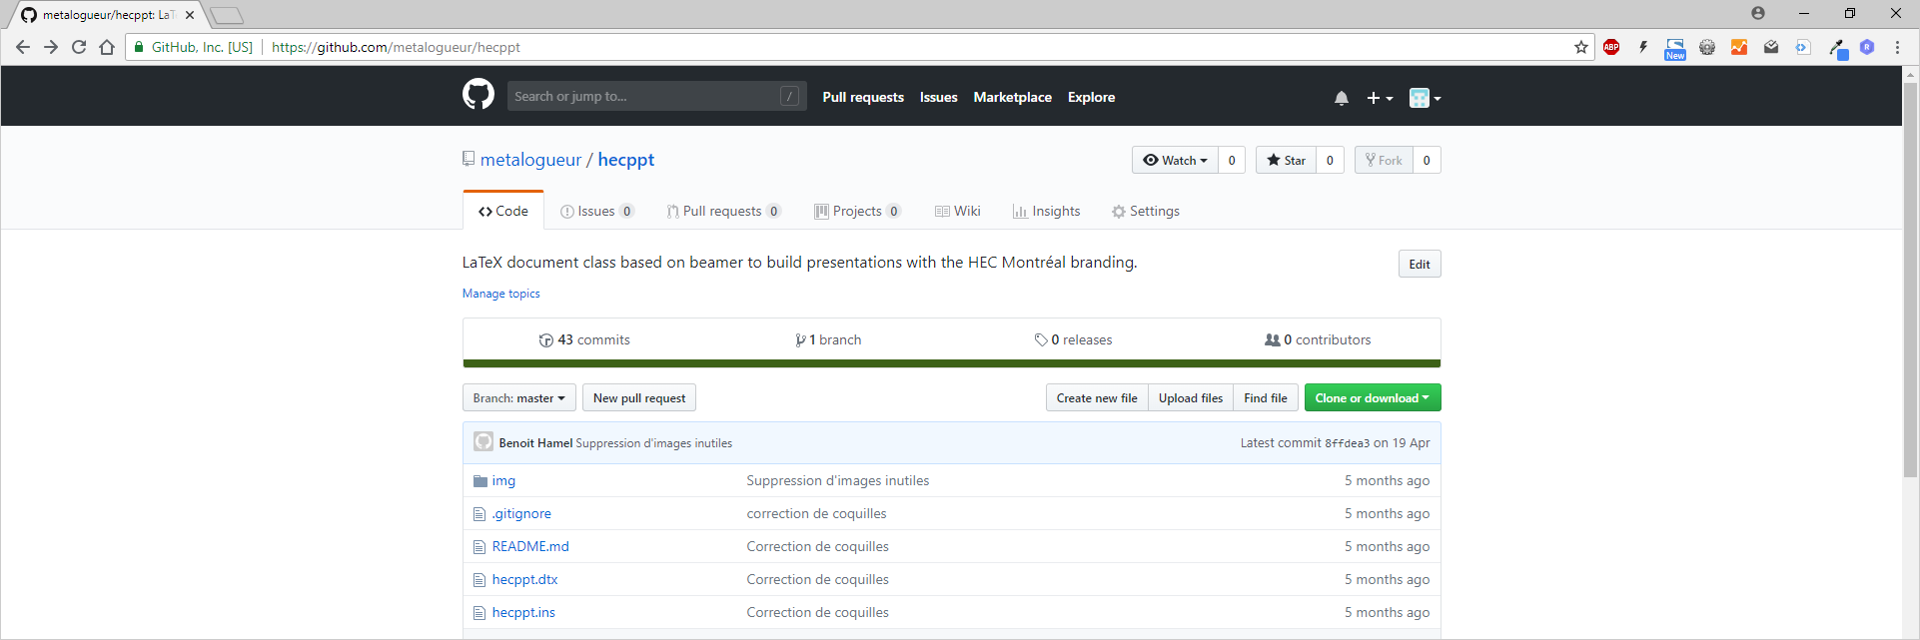
\includegraphics[width=\textwidth]{github-hecppt.png}
			\end{HECimagesstitre}
		
		\end{frame}
		
		\begin{frame}[c]{hecppt document class}
			\framesubtitle{How do we work with it?}
			\begin{itemize}
				\item Download the package from the \HEClien{https://github.com/metalogueur/hecppt/archive/master.zip}{Github repository};
				\item Unzip the archive files in a working directory;
				\item Create your presentation in the \texttt{gabarit.tex} file;
				\item Compile your document.
			\end{itemize}
		\end{frame}
	
\section{Tools available online}
		
		\begin{frame}[c]{Recommended \LaTeX\ tools}
			\begin{itemize}
				\item Recommended \TeX\ distribution: \HEClien{https://www.tug.org/texlive/}{\TeX\ live};
				\item Recommended integrated writing environment: \HEClien{https://www.texstudio.org/}{\TeX\ studio};
				\item Recommended online \LaTeX\ writing tool : \HEClien{https://www.overleaf.com/}{Overleaf}.
			\end{itemize}
		\end{frame}
	
		\begin{frame}[c]{Tutorials}
			\setbeamertemplate{bibliography item}[online]
			
			\begin{thebibliography}{99}
				\bibitem{goulet}
					\HEClien{https://ctan.org/pkg/formation-latex-ul}{formation-latex-ul – Introductory LATEX course in French}
				\bibitem{latex-tuto}
					\HEClien{https://www.latex-tutorial.com/}{\LaTeX -Tutorial.com}
				\bibitem{openclassrooms}
					\HEClien{https://openclassrooms.com/fr/courses/1617396-redigez-des-documents-de-qualite-avec-latex}{OpenClassrooms (French)}
				\bibitem{youtube:krummel}
					\HEClien{https://www.youtube.com/playlist?list=PL1D4EAB31D3EBC449}{\LaTeX\ Tutorials (featuring \TeX maker) [YouTube]}
				\bibitem{overleaf}
					\HEClien{https://www.overleaf.com/latex/learn/free-online-introduction-to-latex-part-1}{Free Online Introduction to \LaTeX}
				\bibitem{lxt30minutes}
					\HEClien{https://www.sharelatex.com/learn/latex/Learn\_LaTeX\_in\_30\_minutes}{Learn \LaTeX\ in 30 minutes}					
			\end{thebibliography}
		\end{frame}
	
		\begin{frame}[c]{Documentation and books}
			\setbeamertemplate{bibliography item}[online]
			
			\begin{thebibliography}{99}
				\bibitem{wikibook}
					\HEClien{https://en.wikibooks.org/wiki/LaTeX}{\LaTeX\ WikiBook}
				\bibitem{sharelatex}
					\HEClien{https://fr.sharelatex.com/learn}{Share\LaTeX\ Documentation}
				\bibitem{ctan}
					\HEClien{https://ctan.org/}{Comprehensive \TeX\ Archive Network}
				\bibitem{uktexfaq}
					\HEClien{http://www.tex.ac.uk/}{UK List of \TeX\ Frequently Asked Questions}
			\end{thebibliography}
		\end{frame}

\section{\LaTeX\ workshops given by the Library}

	\begin{frame}[c]{Beginner workshops}
	
		\begin{itemize}
			\item \LaTeX\ 1 : The Basics (November 1st (French) and 15 (English))
			\begin{itemize}
				\item A brief presentation of \TeX\ and \LaTeX
				\item Document creation
				\item Writing
				\item Document organization
			\end{itemize}
		\end{itemize}
	
		\begin{itemize}
			\item \LaTeX\ 2 : Advanced Notions (November 8 (French) and 22 (English))
			\begin{itemize}
				\item Floating objects (tables and figures)
				\item Maths
				\item Bibliographies and citations
			\end{itemize}
		\end{itemize}
		
	\end{frame}

	\begin{frame}[c]{Specialized workshops}
		
		\begin{itemize}
			\item Coming later, during the Winter 2019 semester\ldots
			\item ``Writing your dissertation with the hecthese document class''
			\item ``Creating presentations with beamer and the hecppt document class''
		\end{itemize}
	\end{frame}
	
\section{Human support}

	\begin{frame}[c]{People who can help you at the library}
		\begin{itemize}
			\item Benoit Hamel, library technician <\href{mailto:benoit.2.hamel@hec.ca}{benoit.2.hamel@hec.ca}>
			\item Mohamed Jabir, data analyst <\href{mailto:mohamed.jabir@hec.ca}{mohamed.jabir@hec.ca}>
			\item Michel Yevenunye Keoula, data analyst <\href{mailto:michel.keoula@hec.ca}{michel.keoula@hec.ca}>
		\end{itemize}
	\end{frame}

\end{document}
